\documentclass[UTF8]{article}
\usepackage[fontset=fandol]{ctex} % Chinese support, using Fandol fonts
\usepackage{graphicx} % Insert images
\usepackage{listings} % Print source code
\usepackage{xcolor} % Color support
\usepackage{booktabs} % Professional table support
\usepackage{pdflscape} % Landscape pages support in PDF
\usepackage{hyperref} % Hypertext links support for cross-referencing
\usepackage{geometry}
\usepackage{enumitem}

% Customize hyperref format (it's set to no special format here)
\hypersetup{hidelinks}

% Declare directories to search for graphics files for graphicx
\graphicspath{{figures/}}

% Define source code style for listings
\lstdefinestyle{c-style}{
  language=C,
  basicstyle=\ttfamily\small\fontfamily{pcr}\selectfont, % 使用 Courier New 字体
  keywordstyle=\bfseries\color{blue},
  identifierstyle=\color{black},
  stringstyle=\color{red},
  commentstyle=\itshape\color{gray},
  backgroundcolor=\color{gray!3},
  numbers=left,
  numberstyle=\tiny\color{gray},
  numbersep=8pt,
  breaklines=true,
  postbreak=\mbox{\textcolor{red}{$\hookrightarrow$}\space},
  frame=single,
  framerule=0.5pt,
  rulecolor=\color{black},
  tabsize=4,
  captionpos=b,
  xleftmargin=15pt,
  xrightmargin=15pt,
  aboveskip=10pt,
  belowskip=10pt,
  showspaces=false,
  showstringspaces=false,
  showtabs=false,
  morekeywords={*,printf,scanf},
  escapeinside={(*@}{@*)}, % 支持代码中插入LaTeX
}

% Define new command for title page
\newcommand{\reporttitle}[2]{
  \LARGE\textsf{#1}\quad\underline{\makebox[12em]{#2}}
}
\newcommand{\reportinfo}[2]{
  \large\makebox[4em]{\textsf{#1}}\quad\underline{\makebox[18em]{#2}}
}

% ----- The document begins here -----
\begin{document}

  % Title page
  \title{Hajimi-OS 作品文档}
  \author{夏彦文 \thanks{学生,计算机学院数据科学与大数据} \and 雷翔麟 \thanks{学生,计算机科学与技术学院}
  \and 邹扬 \thanks{学生,计算机学院数据科学与大数据} \and 潘鹏 \thanks{指导教师,计算机科学与技术学院}}
  \date{\today}
  \maketitle

  % Table of contents
  \newpage
  \tableofcontents
  \newpage

  % Main content
  \section{作品介绍}
    \subsection{项目背景及意义}
    \subsection{国内外研究状况}
    \subsection{项目的主要工作}

  \section{目标理念}

  \section{系统设计与实现}
    \subsection{进程管理}
    进程管理模块的主要功能包括:初始化进程、加载和解析进程、切换进程,以及构建进程状态模块。具体功能介绍如下。
      \subsubsection{进程控制块}
      进程作为操作系统提供的一种抽象层,实际上代表了正在执行的程序。为了便于管理进程,Hajimi-OS采用进程控制块(PCB)来管理操作系统的进程。进程控制块的结构如下所示。
      进程控制块中包含了进程的状态信息,这是操作系统管理进程的基本单元。关于具体的状态,我们将在后文详细解析。
      \lstinputlisting[style=c-style]{processblock.c}
      \subsubsection{进程状态}
      进程状态是一个枚举类型,其定义如下:
      \lstinputlisting[style=c-style]{processstate.c}
      各状态对应如下:
      \begin{enumerate}
        \item UNUSED 状态表示进程控制块未关联任何进程。
        \item SLEEPING 状态表示进程因某种原因暂时未运行。
        \item RUNNABLE 状态表示进程正等待调度器安排运行
        \item RUNNING 状态表示进程正在执行中。
        \item ZOMBIE 状态表示进程已终止,但资源尚未被回收。
      \end{enumerate}
      \subsubsection{分配进程}
      在 Hajimi-OS 中,分配新进程的过程由 allocproc 函数负责。这个函数主要执行以下步骤:
      \begin{enumerate}[label=\textbf{\arabic*}., wide, labelwidth=!, labelindent=0pt]
        \item \textbf{查找 UNUSED 状态的进程控制块:} 系统首先会扫描进程控制块数组,寻找一个状态为 \texttt{UNUSED} 的控制块。如果找到,程序跳转到 \texttt{found} 标签继续操作;如果未找到,则返回 \texttt{NULL},表示当前没有可用的进程控制块,无法创建新进程。
        \item \textbf{初始化进程控制块:} 找到未使用的进程控制块后,函数会分配一个新的进程 ID(通过调用 \texttt{allocpid} 函数),将虚拟内存地址\texttt{vma}设置为 \texttt{NULL},并将内核时间\texttt{ktime}和用户时间\texttt{utime}初始化为 1。
        \item \textbf{分配 trapframe 页面:} 函数为新进程的 trapframe 分配内存(通过调用 \texttt{kalloc} 函数)。如果内存分配失败,函数将释放进程锁并返回 \texttt{NULL}。
        \item \textbf{创建用户和内核页表:} 成功分配 trapframe 页面后,函数创建一个空的用户页表(通过调用 \texttt{proc\_pagetable} 函数)和一个内核页表(通过调用 \texttt{proc\_kpagetable} 函数)。如果任一页表创建失败,函数会清理进程资源并返回 \texttt{NULL}。
        \item \textbf{配置内核堆栈\texttt{kstack}:} 成功分配页表后,函数会设置进程的内核堆栈地址,该地址是预设的虚拟地址。
        \item \textbf{设置新进程的上下文:} 函数初始化进程的上下文\texttt{context},将返回地址寄存器\texttt{ra}设为 \texttt{forkret} 函数地址,堆栈指针\texttt{sp}设为内核堆栈顶部。如此设置后,新进程将从 \texttt{forkret} 函数开始执行。
      \end{enumerate}
      通过这些步骤,allocproc 函数完成了新进程的创建。每个新创建的进程在完成这些步骤后,都会拥有一个唯一的进程 ID,以及自己的页表和堆栈,准备好开始执行。
      \subsubsection{加载和解析进程}
      在 Hajimi-OS 中,除 init 进程外,所有进程都是通过 fork 系统调用进行复制,然后使用 exec 系统调用加载新程序来执行的。
      对于 init 进程,初始化过程如下:
      \begin{enumerate}[label=\textbf{\arabic*}., wide, labelwidth=!, labelindent=0pt]
        \item \textbf{进程分配:} \texttt{Hajimi-OS} 预设了固定数量的进程控制块(Process Control Block,PCB)。每次创建新进程时,系统会在 \texttt{PCB} 数组中寻找一个空闲的块。
        \item \textbf{页表映射:} \texttt{Hajimi-OS} 使用 \texttt{RISC-V} 的 \texttt{sv39} 虚拟内存模型。在此步骤中,操作系统会为程序的各个段(如代码段、数据段等)进行页表映射。我们预先编译了一段二进制代码,专门用于执行 \texttt{init} 程序。 \texttt{init} 程序将使用 \texttt{fork} 系统调用创建一个新进程,然后通过 \texttt{exec} 系统调用执行 \texttt{shell} 程序。原始的 \texttt{init} 进程则会进入无限的进程调度循环。
        \item \textbf{设置进程状态:} 完成以上步骤后,操作系统将进程状态设置为 \texttt{RUNNABLE}。
      \end{enumerate}
      代码如下:
      \lstinputlisting[style=c-style]{processinit.c}
      对于其他进程,其初始化过程大致如下:
      \begin{enumerate}[label=\textbf{\arabic*}., wide, labelwidth=!, labelindent=0pt]
        \item \textbf{使用 \texttt{fork} 系统调用:} \texttt{fork} 的主要功能是生成一个与父进程完全相同的子进程。这个过程包括为新进程创建一个进程控制块(\texttt{PCB}),复制父进程的页表,并在 \texttt{PCB} 中记录父子进程关系,具体存储在 \texttt{PCB} 的 \texttt{parent} 字段中。
        \item \textbf{执行 \texttt{exec} 系统调用:} \texttt{exec} 的主要作用是解析 \texttt{ELF} 文件,并为进程重新映射虚拟内存。通过这种方式,新程序能够在原进程的环境中运行,而不仅仅是复制父进程的行为。这个过程确保了进程的正确创建和程序的正确加载,保证了 \texttt{Hajimi-OS} 的多进程环境能够正常运行。
      \end{enumerate}

      \subsubsection{进程调度}
      目前,Hajimi-OS 操作系统采用时间片均分策略进行进程调度。因此,在时钟中断时,操作系统会中断当前进程并调度下一个进程执行。所有进程的优先级相同,统一放在一个队列中进行调度。接下来,我们将介绍进程切换过程,但首先需要了解 Hajimi-OS 对 CPU 的抽象。

      在 Hajimi-OS 中,CPU 由以下结构体管理,其中关键字段是 proc 和 context。proc 字段指向当前在该 CPU 上运行的进程,而 context 字段用于进程切换。
      \lstinputlisting[style=c-style]{cpustruct.c}
      context 的定义如下:
      \lstinputlisting[style=c-style]{contextstruct.c}
      context 用于保存当前进程的上下文,以便进程下次运行时恢复。Hajimi-OS 的进程调度通过 \texttt{scheduler} 函数实现,当系统需要进行进程切换时,它会扫描所有进程,寻找状态为 RUNNABLE 的进程。

      首先,\texttt{scheduler} 函数从进程列表中选择一个状态为 RUNNABLE 的进程。获取进程后,会锁定该进程以防止其他进程同时修改其状态。

      接下来,将选中的 RUNNABLE 进程状态改为 RUNNING,并将其设置为当前 CPU 正在运行的进程。此时,函数会切换页表到选中进程的内核页表,并刷新地址空间。

      然后,函数执行 \texttt{swtch} 操作,将当前 CPU 的 context 与待运行进程的 context 进行切换。此操作涉及更改处理器的 ra 和 sp 寄存器,使处理器跳转到新进程指定的地址执行,即待运行进程的 ra 寄存器地址。当进程运行结束后,处理器会返回到 \texttt{scheduler} 函数,并将页表切换回内核页表,同时刷新地址空间。此时,进程状态可能已发生变化。

      最后,当前 CPU 的正在运行进程被设置为 0,表示 CPU 暂时没有正在运行的进程。然后释放进程的锁,进行下一轮进程选择。

      如果在一轮循环中没有找到可运行的进程,系统将执行 \texttt{wfi} 指令使处理器进入休眠状态,等待中断唤醒。
      
      \subsubsection{进程释放}
      在 Hajimi-OS 中,当一个进程结束或在进程创建过程中发生错误时,需要释放该进程所占用的资源,这个过程通过 freeproc 函数来完成。该函数的主要步骤如下:
      \begin{enumerate}[label=\textbf{\arabic*}., wide, labelwidth=!, labelindent=0pt]
        \item \textbf{释放 \texttt{trapframe}:} 首先,如果 \texttt{trapframe} 存在,则释放其占用的内存,并将 \texttt{trapframe} 字段设为 0。
        \item \textbf{释放内核页表:} 如果内核页表\texttt{kpagetable}存在,则释放其占用的内存,然后将 \texttt{kpagetable} 字段设为 0。
        \item \textbf{释放用户页表:} 如果用户页表\texttt{pagetable}存在,利用 \texttt{proc\_freepagetable} 函数释放用户页表所占用的内存,同时将 \texttt{pagetable} 字段设为 0。
        \item \textbf{清空进程控制块的其他字段:} 清空进程的虚拟内存地址\texttt{vma},将进程大小\texttt{sz}设为 0,进程 ID\texttt{pid}设为 0,父进程\texttt{parent}设为 0,清空进程的名称\texttt{name},清空等待的条件变量\texttt{chan},设置进程未被杀死(将 \texttt{killed} 设为 0),并将进程的扩展状态设为 0。
        \item \textbf{设置进程状态为 \texttt{UNUSED}:} 最后,将进程状态设为 \texttt{UNUSED},表示该进程控制块可以重新分配给新的进程使用。
      \end{enumerate}
      通过这些步骤,\texttt{freeproc} 函数实现了对进程资源的回收,包括内存资源(如 trapframe、页表等)和进程控制块中的各种字段。回收完毕后,该进程控制块即可被系统重新利用,用于创建新的进程。
    
    \subsection{内存管理}

    
    \subsection{文件系统}

  \section{系统调用的设计实现}

  \section{系统测试}

  \section{总结与展望}

  % \section{实验内容}
  % 一些麻瓜称,根据 NASA 的测算,由于天体运行导致地球的磁场和重力场发生变化,只有在2月10日当天扫帚才可以立起来。
  % 次日,NASA 副局长 Jim Morhard 回应称上述说法不实,基本物理定律每天都有效,并演示了这个实验,如图 \ref{JimMorhard} 所示。

  % % Insert an image, with placement specifier htbp
  % \begin{figure}[htbp]
  %   \centering
  %   
\includegraphics[width=0.5\textwidth]{JimMorhard}
  %   \caption{Jim Morhard 演示立扫帚实验}
  %   \label{JimMorhard}
  % \end{figure}

  % 实验具体要求如下:
  % \begin{enumerate}
  %   \item 扫帚必须能够单独站立,不可以借助其它外力;
  %   \item 实验过程中不得使用咒语,尤其是不得使用永久粘贴咒将扫帚粘在地上。
  % \end{enumerate}

  % \section{实验过程}
  % \subsection{扫帚的选择}
  % 不同的扫帚参数各异,这里列出了部分扫帚的参数,请见表 \ref{broomsticks}。

  % % Insert a three-line table
  % \begin{table}[htbp]
  %   \centering
  %   \begin{tabular}{cccc}
  %     \toprule
  %     序号 & 名称 & 上市时间 & 最高时速 \\
  %     \midrule
  %     1 & 彗星290 & 1995年 & 60\,mph \\
  %     2 & 光轮1000 & 1967年 & 100\,mph \\
  %     3 & 光轮2001 & 1992年 & >\,100\,mph \\
  %     4 & 火弩箭 & 1993年 & 150\,mph \\
  %     \bottomrule
  %   \end{tabular}
  %   \caption{部分扫帚的参数对比}
  %   \label{broomsticks}
  % \end{table}

  % 但是,本次实验不是魁地奇比赛,扫帚的最高时速对实验的进行没有太大的影响。
  % 为了选出合适的扫帚,这里采用随机抽签的办法,编写了一个 C 程序进行抽取:

  % % Insert source code
  % \lstinputlisting[style=c-style]{random.c}

  % % Insert an image in a separate landscape page
  % \begin{landscape}
  %   \begin{figure}
  %     \centering
  %     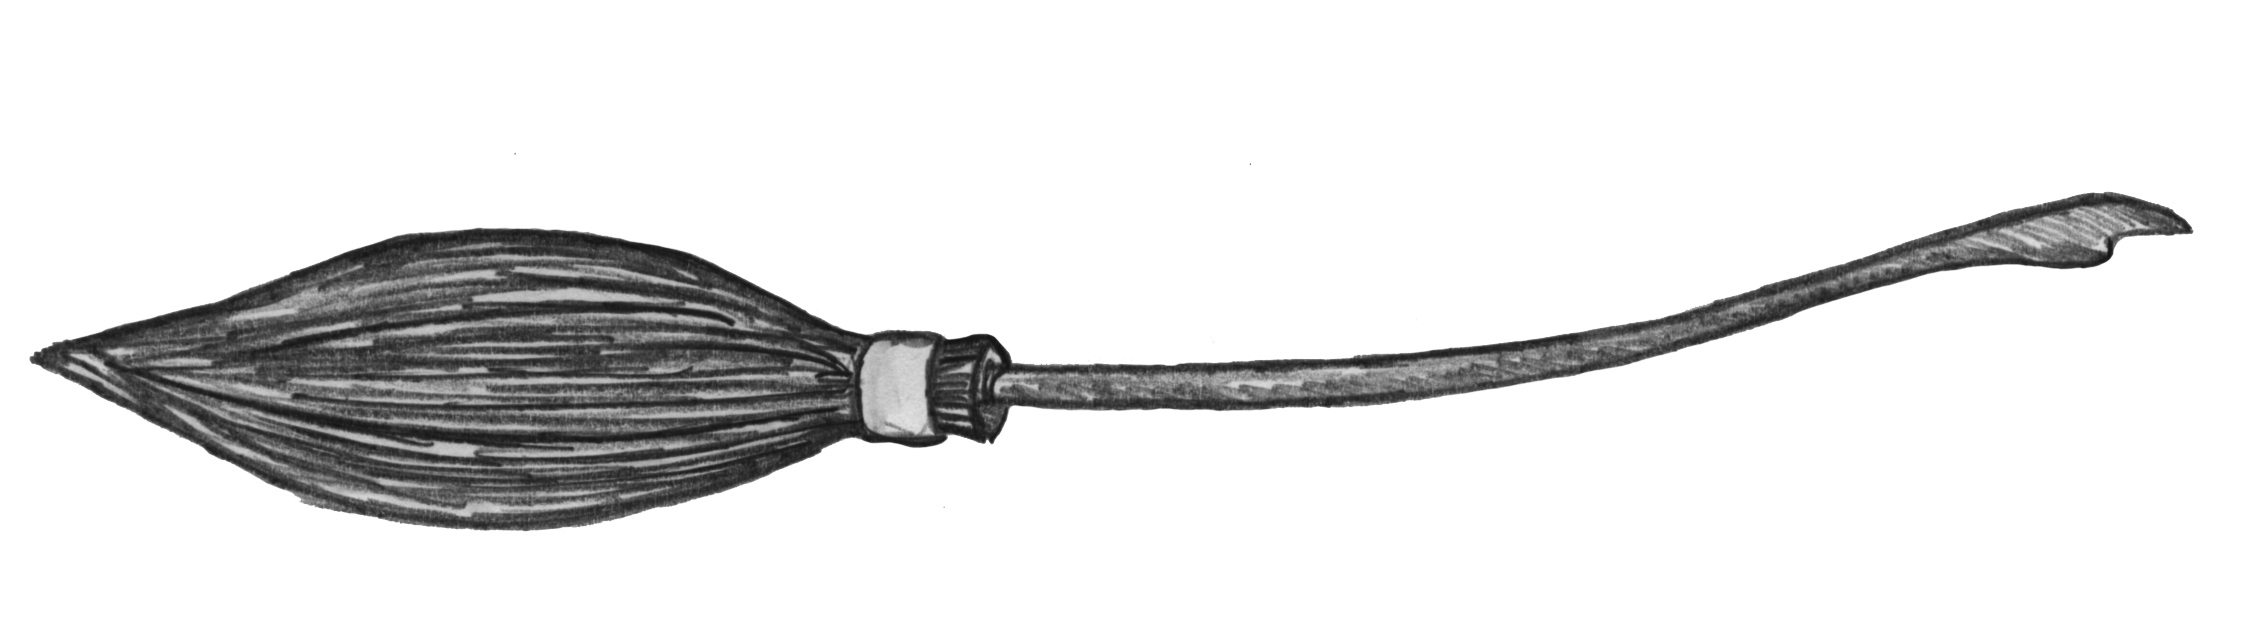
\includegraphics[width=\linewidth]{Nimbus2001}
  %     \caption{光轮2001扫帚}
  %     \label{Nimbus2001}
  %   \end{figure}
  % \end{landscape}

  % 为了解决上述问题,我在实验中采用了先将扫帚毛从中间稍稍分开,用手扶着竖直立在地上后,再进行调整的方式。
  % 调整的过程中,先将扫帚向扫帚柄弯曲的反方向旋转一定角度以抵消弯曲的扫帚柄产生的影响,之后再不断尝试进行微调。
  % 经过近 10 分钟的不懈努力,扫帚被成功立起。

  % \section{实验总结}
  % 本次实验中,扫帚被成功立起,证实了在不使用魔法的情况下,基本物理定律在霍格沃茨仍然适用。
\end{document}
